\section{Attitude Model}
The model of the quadcopter is split into two sub models as presented previously. One of the sub models is the attitude model, that describes the angles of pitch, roll and yaw. The attitude model is now derived.


Free body diagrams are illustrated in \autoref{fig:diagramQuad} and \autoref{fig:diagramTorque}. 

%\begin{figure}[H]
%\centering
%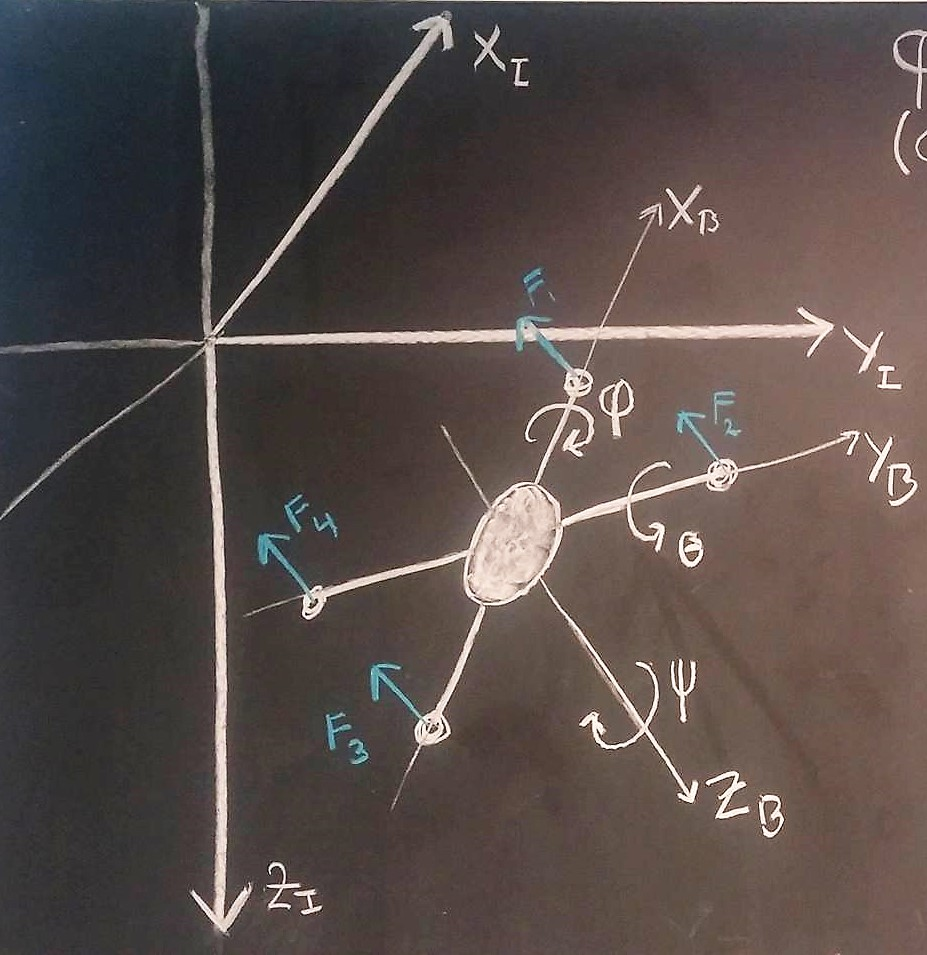
\includegraphics[scale=.27]{figures/drone_diagram}
%
%
%\caption{Free body diagram that holds both the inertial and body reference systems, as well as the references for the angles roll, pitch and yaw.}
%\label{fig:diagramQuad}
%\end{figure}

\begin{minipage}{\linewidth}
	\begin{minipage}{0.45\linewidth}
		\begin{figure}[H]
			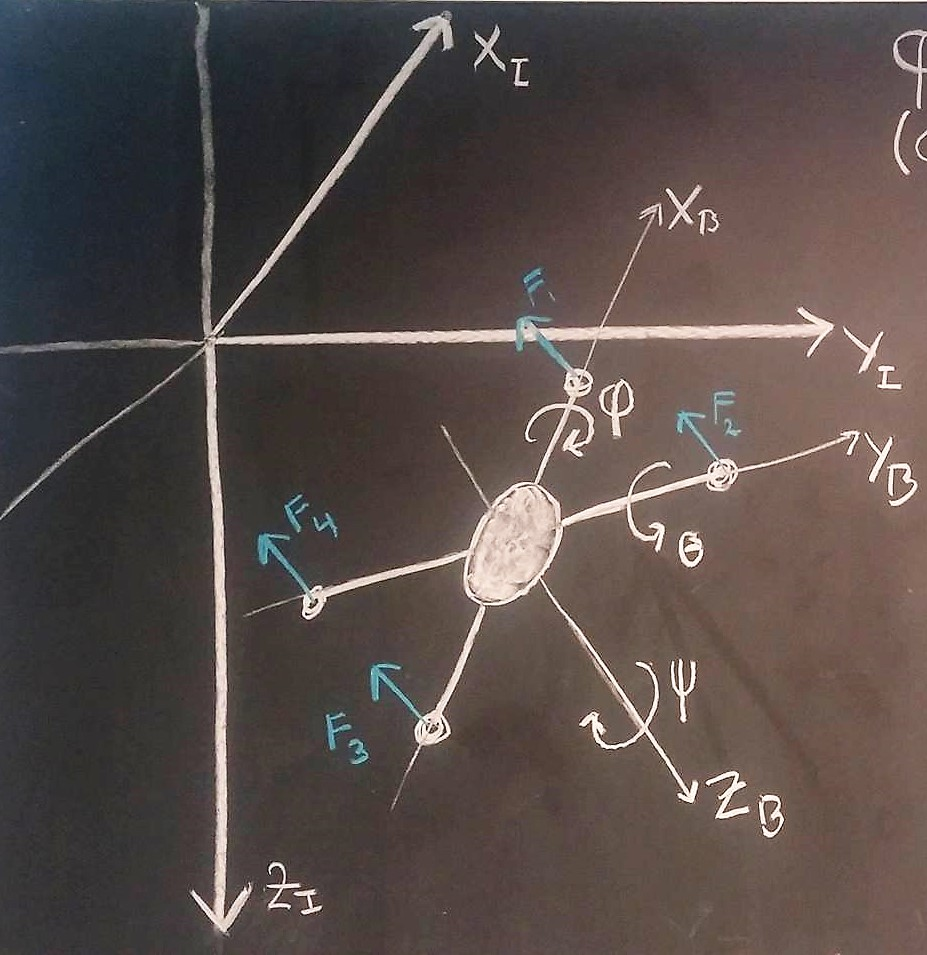
\includegraphics[scale=.27]{figures/drone_diagram}
			\centering
			
			\captionof{figure}{Free body diagram that holds both the inertial and body reference systems, as well as the references for the angles roll, pitch and yaw.}
			\label{fig:diagramQuad}
		\end{figure}
	\end{minipage}
	\hspace{0.03\linewidth}
	\begin{minipage}{0.45\linewidth}
		\begin{figure}[H] \vspace{16mm}
			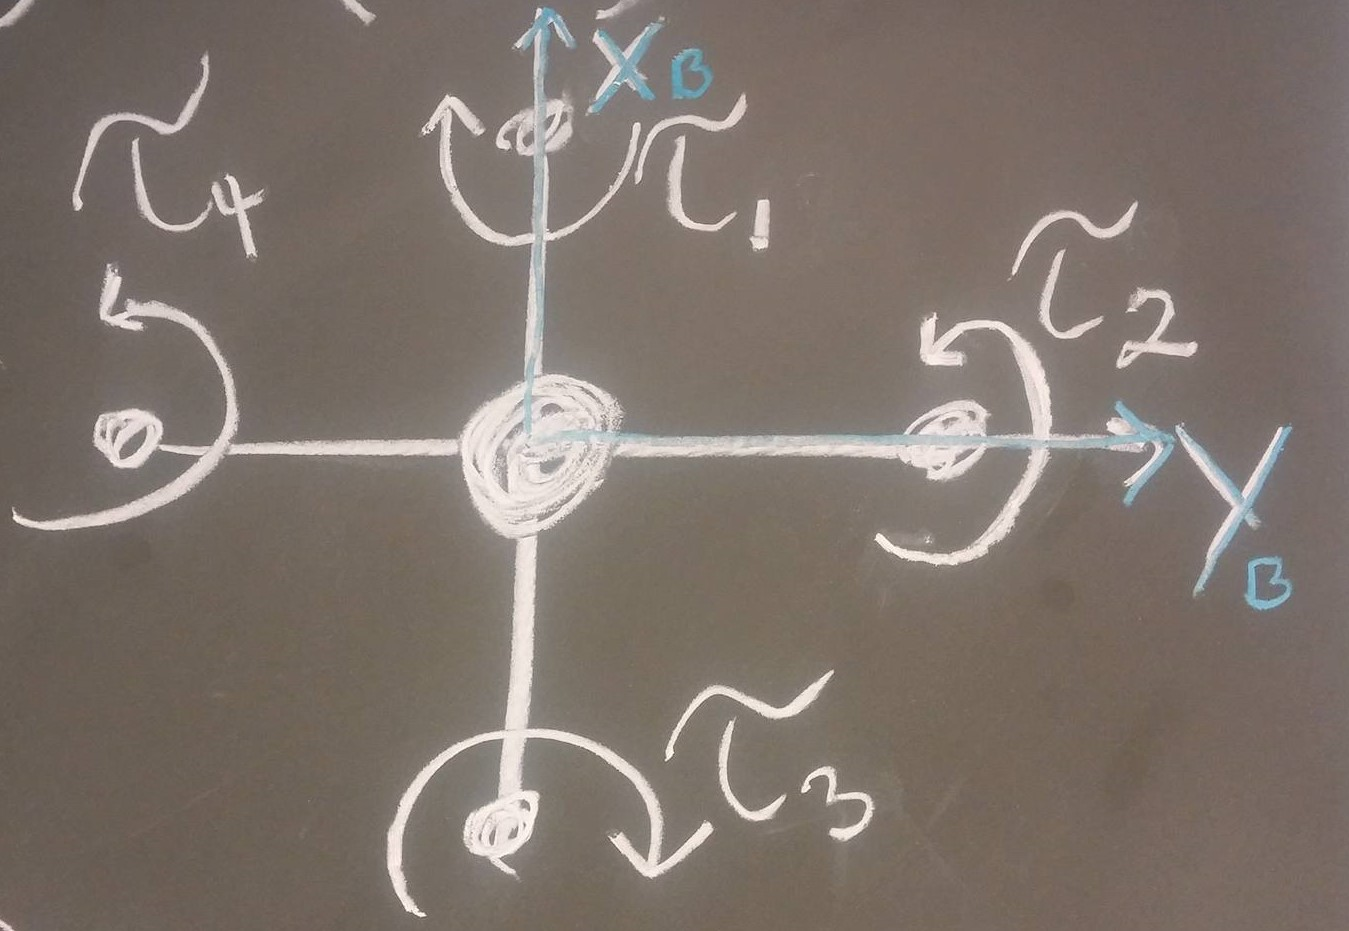
\includegraphics[scale=.18]{figures/torques_diagram}
			\centering
			\captionof{figure}{Free body diagram with the references for the torques produced by the drag force at the propeller.}
			\label{fig:diagramTorque}
		\end{figure}
	\end{minipage}
\end{minipage}


From the diagrams above, the equations of angular motion along the three body axes can be derived.
%
\begin{align}
	J_x\cdot\ddot{\phi}&=(F_4-F_2)\cdot L &\\
	J_y \cdot\ddot{\theta}&=(F_1-F_3)\cdot L &\\
	J_z\cdot\ddot{\psi}&=\tau_1-\tau_2+\tau_3-\tau_4
	\label{eq:AngleEq}
\end{align}

\begin{where}
\va{\ddot{\phi}}{is roll angular acceleration}{rad $\cdot$ s$^{-2}$}\\

\end{where}




\hspace{6mm} Where:\\
\begin{tabular}{ p{1cm} l l l}
	& \si{\ddot{\phi}} 	 	& is roll angular acceleration   	&\unitWh{rad \cdot s^{-2}} \\
	& \si{\ddot{\theta}} 	& is  pitch angular acceleration   &\unitWh{rad \cdot s^{-2}} \\
	& \si{\ddot{\psi}}	    & is yaw angular acceleration      &\unitWh{rad \cdot s^{-2}} \\
	& \si{J_x}  			& is the body moment of inertia around \si{x_B} direction       &\unitWh{kg \cdot m^2} \\
	& \si{J_y}          	& is the body moment of inertia around \si{y_B} direction        &\unitWh{kg \cdot m^2} \\
	& \si{J_z}          	& is the body moment of inertia around \si{z_B} direction        &\unitWh{kg \cdot m^2} \\	
	& \si{L}  				& is the length of the arm of the quadcopter      &\unitWh{m} \\
	& \si{F_n}          	& is the thrust force produced in each propeller        &\unitWh{N} \\
	& \si{\tau_n}          	& is the torque due to the drag force in each propeller        &\unitWh{N \cdot m} \\		
\end{tabular}

As it can be seen in the \eqref{eq:AngleEq}, the roll and pitch angular accelerations depend on the thrust forces exerted by the propellers placed in the y and x axes of the quadcopter, respectively. The yaw angle changes only due to the torques created by the drag force in the propeller.

The thrust forces and drag torques from the propeller can be approximated by terms depending on the velocity of the motor, which are found as described in Appendix \ref{}. The equations above can be rewritten to include these terms.
%
\begin{flalign}
	\eq{ J_x\cdot\ddot{\phi} }{k_{th} \cdot(\omega^2_4-\omega^2_2) \cdot L} &\\
	\eq{J_y \cdot\ddot{\theta}}{k_{th} \cdot(\omega^2_1-\omega^2_3) \cdot L} &\\
	\eq{J_z\cdot\ddot{\psi}}{k_d \cdot(\omega^2_1-\omega^2_2+\omega^2_3-\omega^2_4)}
	\label{eq:AngleEqVelocities}
\end{flalign}
%
\hspace{6mm} Where:\\
\begin{tabular}{ p{1cm} l l l}	
	& \si{k_{th}}  			& is the thrust constant      					&\unitWh{N \cdot s^2 \cdot m^{-2}} \\
	& \si{k_d}          	& is the drag constant        					&\unitWh{N \cdot m \cdot s^2 \cdot m^{-2}} \\
	& \si{\omega_n}         & is the angular velocity of the nth motor      &\unitWh{rad \cdot s^{-1}}	
\end{tabular}